%%%%%%%%%%%%%%%%%%%%%%%%%%%%%%%%%%%%%%%%%
% Beamer Presentation
% LaTeX Template
% Version 1.0 (10/11/12)
%
% This template has been downloaded from:
% http://www.LaTeXTemplates.com
%
% License:
% CC BY-NC-SA 3.0 (http://creativecommons.org/licenses/by-nc-sa/3.0/)
%
%%%%%%%%%%%%%%%%%%%%%%%%%%%%%%%%%%%%%%%%%

%----------------------------------------------------------------------------------------
%	PACKAGES AND THEMES
%----------------------------------------------------------------------------------------

\documentclass{beamer}
\usepackage{multicol}
\usepackage{xcolor}
\usepackage{listings}

\definecolor{applegreen}{rgb}{0.55, 0.71, 0.0}
\definecolor{blue(ncs)}{rgb}{0.0, 0.53, 0.74}
\definecolor{burgundy}{rgb}{0.5, 0.0, 0.13}

\mode<presentation> {

\usetheme{CambridgeUS}

\usecolortheme{wolverine}

\definecolor{gold}{HTML}{D4A017}
\definecolor{darkgold}{HTML}{B7950B}

\setbeamercolor{palette primary}{bg=gold,fg=white}
\setbeamercolor{palette secondary}{bg=darkgold,fg=white}
\setbeamercolor{palette tertiary}{bg=black,fg=white}
\setbeamercolor{palette quaternary}{bg=gold,fg=white}

\setbeamercolor{frametitle}{bg=darkgold,fg=white}

\setbeamercolor{section number projected}{bg=black,fg=gold}
\setbeamercolor{item}{fg=black,bg=gold}
}

\usepackage{graphicx} % Allows including images
\usepackage{booktabs} % Allows the use of \toprule, \midrule and \bottomrule in tables

%----------------------------------------------------------------------------------------
%	TITLE PAGE
%----------------------------------------------------------------------------------------

\title[Generic Finite Element Interfaces]{On Performance and Portability for\\Generic Finite Element Interfaces} % The short title appears at the bottom of every slide, the full title is only on the title page

\author{Jeremy L Thompson} % Your name
\institute[CU Boulder] % Your institution as it will appear on the bottom of every slide, may be shorthand to save space
{University of Colorado Boulder \\ % Your institution for the title page
\medskip
\textit{jeremy.thompson@colorado.edu} % Your email address
}
\date{\today} % Date, can be changed to a custom date

\begin{document}

\begin{frame}
\titlepage % Print the title page as the first slide
\end{frame}

%------------------------------------------------

\begin{frame}
\begin{center}
\frametitle{Overview}

A global sparse matrix is no longer a good representation of a\\high-order linear operator\\

~\\

libCEED is an extensible library that provides a portable\\algebraic interface and optimized implementations\\

~\\

We have preliminary results comparing performance to native implementations in production software

\end{center}
\end{frame}
 
%------------------------------------------------

\begin{frame}
\frametitle{Overview} % Table of contents slide, comment this block out to remove it
\tableofcontents % Throughout your presentation, if you choose to use \section{} and \subsection{} commands, these will automatically be printed on this slide as an overview of your presentation
\end{frame}

%----------------------------------------------------------------------------------------
%	PRESENTATION SLIDES
%----------------------------------------------------------------------------------------

%------------------------------------------------
\section{Introduction}
%------------------------------------------------

\begin{frame}
\begin{center}
\frametitle{Weak Form and Finite Elements}

\begin{itemize}

\item Strong Form of PDE: $A_s u = f$\\

~\\

\item Weak Form of PDE: $\int_\Omega A u v = \int_\Omega f v$\\

~\\

\item $v$ are test functions defined on each element,\\

\hspace{6mm} yields system of equations

~\\

\item Operator can be decomposed algebraically

\end{itemize}

\end{center}
\end{frame}

%------------------------------------------------

\begin{frame}
\begin{center}
\frametitle{Operator Decomposition}

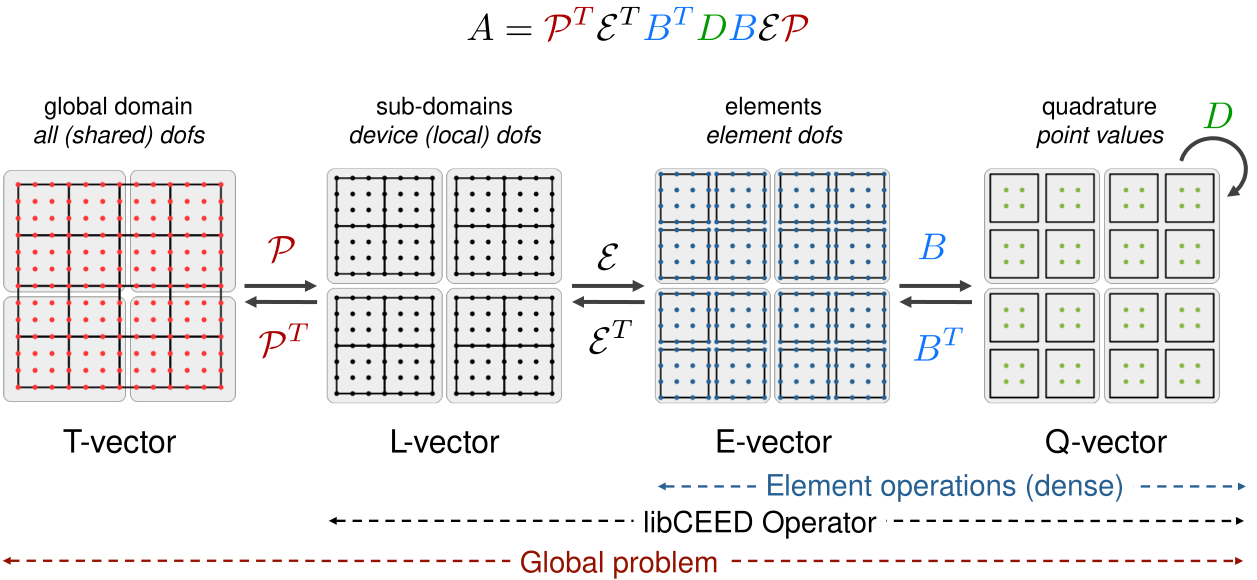
\includegraphics[width=11cm]{libCEEDAPI}

\end{center}
\end{frame}

%------------------------------------------------

\begin{frame}
\begin{center}
\frametitle{Matrix Free Implementation}

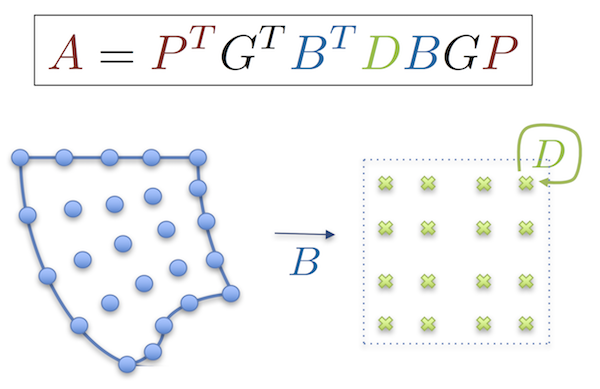
\includegraphics[width=5cm]{libCEEDRefElm}

\begin{itemize}

\item Avoid global matrix assembly

\item Map each element to reference element

\item Only store map to reference, action on reference

\item Easy to parallelize across nodes

\end{itemize}

\end{center}
\end{frame}

%------------------------------------------------
\section{libCEED}
%------------------------------------------------

\begin{frame}
\begin{center}
\frametitle{libCEED API}

\begin{itemize}

\item Provides on-device operator implementation\\

~\\

\item Easy to incorporate into existing code\\

~\\

\item Supports multiple types of computational devices\\

\hspace{6mm} GPUs, CPUs, etc\\

~\\

\item Multiple extensible implementations\\

\hspace{6mm} Reference on CPUs, OCCA on GPUs

\end{itemize}

\end{center}
\end{frame}

%------------------------------------------------

\begin{frame}
\begin{center}
\frametitle{API Objects}

\begin{itemize}

\item $G$ - CeedRestriction\\

\hspace{6mm} Restrict to single element\\

~\\

\item {\color{blue(ncs)} $B$} - CeedBasis\\

\hspace{6mm} Actions on basis such as interpolation,\\

\hspace{6mm} gradient, divergence, curl

~\\

\item {\color{applegreen} $D$} - CeedQFunction\\

\hspace{6mm} Operator action at quadrature points\\

\hspace{6mm} to include coefficient functions

\end{itemize}

\end{center}
\end{frame}

%------------------------------------------------

\begin{frame}
\begin{center}
\frametitle{Device Level Operator}

\begin{itemize}

\item $L = G^T {\color{blue(ncs)} B^T} {\color{applegreen} D} {\color{blue(ncs)} B} G$ - CeedOperator\\

~\\

\item libCEED objects are combined to create a CeedOperator\\

~\\

\item CeedOperator gives operator action for elements on device\\

~\\

\item User code responsible for communication between devices\\

\hspace{6mm} $A = {\color{burgundy} P^T} L {\color{burgundy} P}$

\end{itemize}

\end{center}
\end{frame}


%------------------------------------------------

\begin{frame}
\begin{center}
\frametitle{Benefits}

\begin{itemize}

\item Extensible library\\

~\\

\item Lower memory transfer, no sparse matrix\\

~\\

\item Implementations for multiple devices and backends\\

~\\

\item libCEED optimization can benefit all operators\\

\hspace{6mm} Tensor contraction, basis application, etc

\end{itemize}

\end{center}
\end{frame}

%------------------------------------------------
\section{Production Software}
%------------------------------------------------

\begin{frame}[fragile]
\begin{center}
\frametitle{Standalone Implementation}

\begin{lstlisting}[language=C]
// Solve system
if (mpi_rank == 0) {
	globalCGSolve(global_vector, f_vector,
	boundary_vector);
}
else if (mpi_rank > 3) {
	localOperatorApply(&ceed,
	&processor_operator);
}
\end{lstlisting}



\end{center}
\end{frame}

%------------------------------------------------

\begin{frame}[fragile]
\begin{center}
\frametitle{MFEM}

{\small
\begin{lstlisting}[language=c++]
/// Wrapper for a mass CeedOperator as an
/// mfem::Operator
class CeedMassOperator : public mfem::Operator
 protected:
  const mfem::FiniteElementSpace *fes;
  CeedOperator build_oper, oper;
  CeedBasis basis, mesh_basis;
  CeedElemRestriction restr, mesh_restr;
  CeedQFunction apply_qfunc, build_qfunc;
  CeedVector node_coords, qdata;

\end{lstlisting}
}

\end{center}
\end{frame}

%------------------------------------------------

\begin{frame}[fragile]
\begin{center}
\frametitle{Nek5000}

{\small
\begin{lstlisting}[language=Fortran]
subroutine ceed_axhm1(pap,ap1,p1,h1,h2,ceed,op_mass,
$ vec_ap1,vec_p1,vec_qdata)

include 'ceedf.h'

c Vector conjugate gradient matvec for solution of 
c uncoupled Helmholtz equations

include 'SIZE'
include 'TOTAL'
...
call ceedvectorsetarray(vec_p1,ceed_mem_host,
$ ceed_use_pointer, p1,err)
call ceedoperatorapply(op_mass,vec_qdata,vec_p1,vec_ap1,
$ ceed_request_immediate,err)
call ceedvectorgetarray(vec_ap1,ceed_mem_host,ap1,err)
\end{lstlisting}
}

\end{center}
\end{frame}

%------------------------------------------------

\begin{frame}[fragile]
\begin{center}
\frametitle{PETSc}

{\small
\begin{lstlisting}[language=C]
user->op = op_mass;
user->qdata = qdata;

ierr = MatCreateShell(comm, mdof[0]*mdof[1]*mdof[2],
       mdof[0]*mdof[1]*mdof[2],
       PETSC_DECIDE, PETSC_DECIDE, user, &mat);
CHKERRQ(ierr);
ierr = MatShellSetOperation(mat, MATOP_MULT
       (void(*)(void))MatMult_Mass); CHKERRQ(ierr);

...

ierr = KSPSetFromOptions(ksp); CHKERRQ(ierr);
ierr = KSPSetOperators(ksp, mat, mat); CHKERRQ(ierr);
ierr = KSPSolve(ksp, rhs, X); CHKERRQ(ierr);
\end{lstlisting}
}

\end{center}
\end{frame}

%------------------------------------------------
\section{Performance Comparison}
%------------------------------------------------

\begin{frame}
\begin{center}
\frametitle{Nek5000}


\includegraphics[height=1.5cm]{libCEEDCURCLogo}

\begin{flushleft}

\begin{multicols}{2}

Problem: $\nabla u = f$\\

\hspace{2mm} CEED Benchmark Problem 1\\

~\\

Domain: 3D Cube\\

Elements: Hexagonal\\

Number of Elements: $2^n$\\

Shape Function Order: $7$\\

Quadrature Order: $8$\\

Computer: CU Boulder Summit\\

~\\

~\\

Nodes: 1\\

CPUs: Intel Xeon Haswell\\

Processors: 32\\

Compiler: Intel/17.0.0\\

MPI: Intel/2017.0.098

\end{multicols}

\end{flushleft}

\end{center}
\end{frame}

%------------------------------------------------

\begin{frame}
\begin{center}
\frametitle{Nek5000 - The Good News}

\begin{multicols}{2}

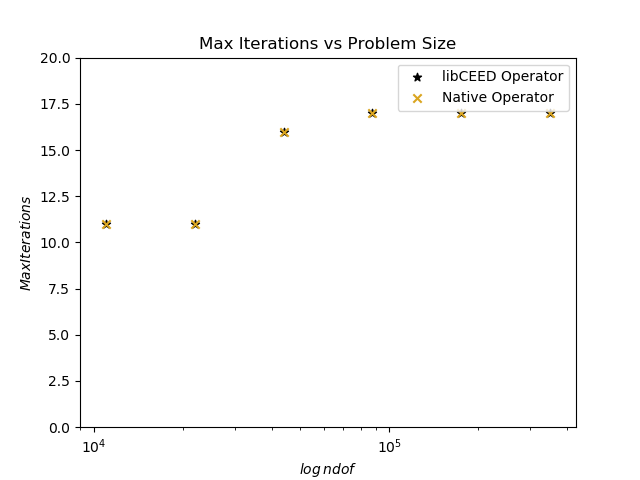
\includegraphics[width=6.2cm]{libCEEDmaxItrVsSize}

~\\

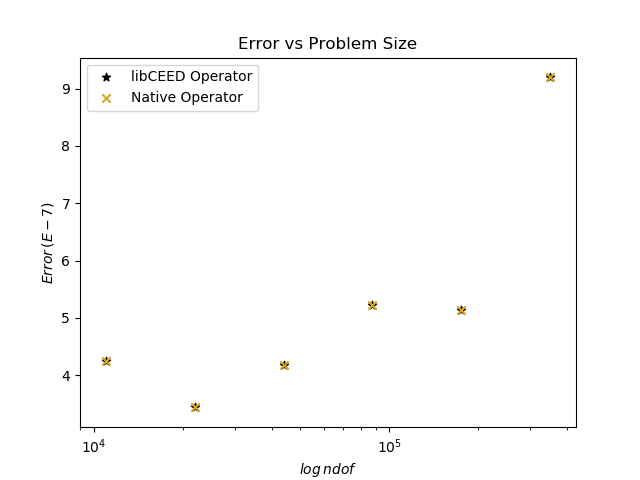
\includegraphics[width=6.2cm]{libCEEDerrorVsSize}

\end{multicols}

\end{center}
\end{frame}

%------------------------------------------------

\begin{frame}
\begin{center}
\frametitle{Nek5000 - The Bad News}

\begin{multicols}{2}

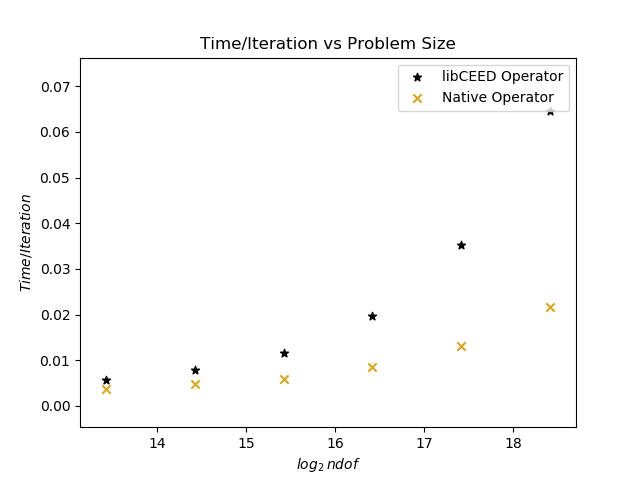
\includegraphics[width=6.2cm]{libCEEDitrTimeVsSize}

~\\

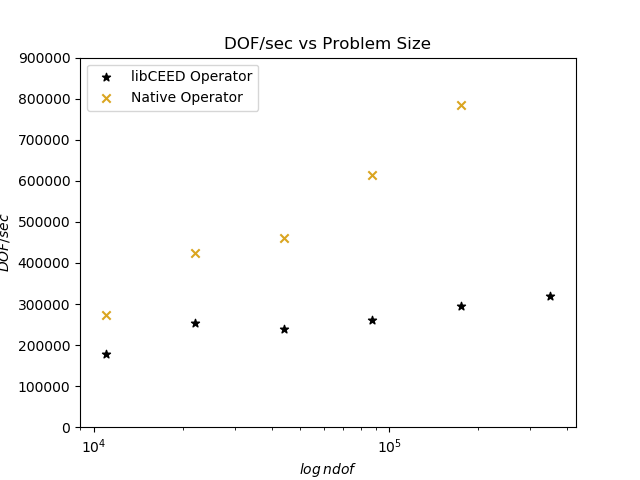
\includegraphics[width=6.2cm]{libCEEDdofSecVsSize}

\end{multicols}

\end{center}
\end{frame}

%------------------------------------------------

\begin{frame}
\begin{center}
\frametitle{Future Work}

\begin{itemize}

\item Optimize reference implementation, tensor contraction\\

~\\

\item Create library of user quadrature functions\\

~\\

\item Create additional backends\\

~\\

\item Compare libCEED operators to native implementation in a\\ wider range of production software

\end{itemize}

\end{center}
\end{frame}

%------------------------------------------------
\section{Questions}
%------------------------------------------------

\begin{frame}
\begin{center}
\frametitle{Questions?}

{\flushleft

Advisor: \hspace{8mm} Jed Brown\textsuperscript{1}\\

~\\

Collaborators: Jean-Sylvain Camier\textsuperscript{2}, Tzanio Kolev\textsuperscript{2},\\
\hspace{23mm} Veselin Dobrev\textsuperscript{2}, \& Thilina Rathnayake\textsuperscript{3}\\

~\\

Grant: \hspace{11mm} Exascale Computing Project (17-SC-20-SC)\\

~\\

~\\

\small{1: University of Colorado, Boulder\\
2: Lawrence Livermore National Laboratory\\
3: University of Illinois, Urbana-Champaign\\}}

\end{center}
\end{frame}

%------------------------------------------------

\begin{frame}[noframenumbering]
\titlepage % Print the title page
\end{frame}

%------------------------------------------------

%----------------------------------------------------------------------------------------

\end{document} 